\documentclass[]{article}
\usepackage{lmodern}
\usepackage{amssymb,amsmath}
\usepackage{ifxetex,ifluatex}
\usepackage{fixltx2e} % provides \textsubscript
\ifnum 0\ifxetex 1\fi\ifluatex 1\fi=0 % if pdftex
  \usepackage[T1]{fontenc}
  \usepackage[utf8]{inputenc}
\else % if luatex or xelatex
  \ifxetex
    \usepackage{mathspec}
  \else
    \usepackage{fontspec}
  \fi
  \defaultfontfeatures{Ligatures=TeX,Scale=MatchLowercase}
\fi
% use upquote if available, for straight quotes in verbatim environments
\IfFileExists{upquote.sty}{\usepackage{upquote}}{}
% use microtype if available
\IfFileExists{microtype.sty}{%
\usepackage{microtype}
\UseMicrotypeSet[protrusion]{basicmath} % disable protrusion for tt fonts
}{}
\usepackage[margin=1in]{geometry}
\usepackage{hyperref}
\hypersetup{unicode=true,
            pdftitle={Supplementary materials: Orienting the causal relationship between imprecisely measured traits using GWAS summary data},
            pdfborder={0 0 0},
            breaklinks=true}
\urlstyle{same}  % don't use monospace font for urls
\usepackage{graphicx,grffile}
\makeatletter
\def\maxwidth{\ifdim\Gin@nat@width>\linewidth\linewidth\else\Gin@nat@width\fi}
\def\maxheight{\ifdim\Gin@nat@height>\textheight\textheight\else\Gin@nat@height\fi}
\makeatother
% Scale images if necessary, so that they will not overflow the page
% margins by default, and it is still possible to overwrite the defaults
% using explicit options in \includegraphics[width, height, ...]{}
\setkeys{Gin}{width=\maxwidth,height=\maxheight,keepaspectratio}
\IfFileExists{parskip.sty}{%
\usepackage{parskip}
}{% else
\setlength{\parindent}{0pt}
\setlength{\parskip}{6pt plus 2pt minus 1pt}
}
\setlength{\emergencystretch}{3em}  % prevent overfull lines
\providecommand{\tightlist}{%
  \setlength{\itemsep}{0pt}\setlength{\parskip}{0pt}}
\setcounter{secnumdepth}{0}
% Redefines (sub)paragraphs to behave more like sections
\ifx\paragraph\undefined\else
\let\oldparagraph\paragraph
\renewcommand{\paragraph}[1]{\oldparagraph{#1}\mbox{}}
\fi
\ifx\subparagraph\undefined\else
\let\oldsubparagraph\subparagraph
\renewcommand{\subparagraph}[1]{\oldsubparagraph{#1}\mbox{}}
\fi

%%% Use protect on footnotes to avoid problems with footnotes in titles
\let\rmarkdownfootnote\footnote%
\def\footnote{\protect\rmarkdownfootnote}

%%% Change title format to be more compact
\usepackage{titling}

% Create subtitle command for use in maketitle
\newcommand{\subtitle}[1]{
  \posttitle{
    \begin{center}\large#1\end{center}
    }
}

\setlength{\droptitle}{-2em}
  \title{Supplementary materials: Orienting the causal relationship between
imprecisely measured traits using GWAS summary data}
  \pretitle{\vspace{\droptitle}\centering\huge}
  \posttitle{\par}
  \author{}
  \preauthor{}\postauthor{}
  \predate{\centering\large\emph}
  \postdate{\par}
  \date{28 July 2017}

\begin{document}
\maketitle

\subsection{Supplementary text 1}\label{supplementary-text-1}

We assume the following model

\[
\begin{aligned}
x   & = \alpha_g + \beta_g g + \epsilon_g \\
x_o & = \alpha_{mx} + \beta_{mx} x + \epsilon_{mx} \\
y   & = \alpha_x + \beta_x x + \epsilon_x \\
y_o & = \alpha_{my} + \beta_{my} y + \epsilon_{my}
\end{aligned}
\]

where \(x\) is the exposure on the outcome \(y\), \(g\) is an instrument
that has a direct effect on \(x\), \(x_o\) is the measured quantity of
\(x\), where measurement error is incurred from linear transformation in
\(\alpha_{mx}\) and \(\beta_{mx}\) and imprecision from
\(\epsilon_{mx}\), and \(y_o\) is the measured quantity of \(y\), where
measurement error is incurred from linear transformation in
\(\alpha_{my}\) and \(\beta_{my}\) and imprecision from
\(\epsilon_{my}\). Our objective is to estimate the expected magnitude
of association between \(g\) and \(y\) after conditioning on \(x\).
Under the CIT, this is expected to be \(cov(g, y_o - \hat{y}_o) = 0\)
when \(x\) causes \(y\), where
\(\hat{y}_o = \hat{a}_{x_o} + \hat{\beta}_{x_o} x_o\) is the predicted
value of \(y_o\) using the measured value of \(x_o\).

We can split \(cov(g, y_o - \hat{y}_o)\) into two parts, \(cov(g, y_o)\)
and \(cov(g, \hat{y}_o)\).

\textbf{Part 1}

\[
\begin{aligned}
cov(g, y_o) & = cov(g, \beta_{my} y) \\
            & = cov(g, \beta_{my} \beta_x x) \\
            & = cov(g, \beta_{my} \beta_x \beta_g g) \\
            & = \beta_{my} \beta_x \beta_g var(g)
\end{aligned}
\]

\textbf{Part 2}

\[
\begin{aligned}
cov(g, \hat{y}_o) & = cov(g, \hat{\beta}_{x_o} x_o) \\
                  & = cov(g, \hat{\beta}_{x_o} \beta_{mx} x) \\
                  & = cov(g, \hat{\beta}_{x_o} \beta_{mx} \beta_g g) \\
                  & = \hat{\beta}_{x_o} \beta_{mx} \beta_g var(g)
\end{aligned}
\]

Simpifying further

\[
\begin{aligned}
\hat{\beta}_{x_o} & = \frac{cov(y_o, x_o)} {var(x_o)} \\
                  & = \frac{cov(\beta_{my} y, \beta_{mx} x)} {\beta_{mx}^2 var(x) + var(\epsilon_{mx})} \\
                  & = \frac{\beta_{mx} \beta_{my} cov(y, x)} {\beta_{mx}^2 var(x) + var(\epsilon_{mx})} \\
                  & = \frac{\beta_{mx} \beta_{my} \beta_x var(x)} {\beta_{mx}^2 var(x) + var(\epsilon_{mx})}
\end{aligned}
\]

which can be substituted back to give

\[
\begin{aligned}
cov(g, \hat{y}_o) & = \frac{\beta_{my} \beta_x \beta_g var(g) \beta_{mx}^2 var(x)} {\beta_{mx}^2 var(x) + var(\epsilon_{mx})} \\
                  & = \frac{\beta_{mx}^2 var(x)} {\beta_{mx}^2 var(x) + var(\epsilon_{mx})} \times \beta_{my} \beta_x \beta_g var(g)
\end{aligned}
\]

Finally

\[
\begin{aligned}
cov(g, y_o - \hat{y}_o) & = \beta_{my} \beta_x \beta_g var(g) - \frac{\beta_{mx}^2 var(x)} {\beta_{mx}^2 var(x) + var(\epsilon_m)} \times \beta_{my} \beta_x \beta_g var(g)
\end{aligned}
\]

thus \(cov(g, y_o - \hat{y}_o) = 0\) if the measurement imprecision in
\(x_o\) is \(var(\epsilon_m) = 0\). However if there is any imprecision
then the condition \(cov(g, y_o - \hat{y}_o) = 0\) will not hold.

\newpage

\subsection{Supplementary text 2}\label{supplementary-text-2}

Assuming that either \(x \rightarrow y\) or \(y \rightarrow x\), the
causal direction can be inferred by evaluating which of \(\rho_{g, x}\)
and \(\rho_{g, y}\) is larger in magnitude. The Steiger test is a
hypothesis test that provides a p-value for observing the difference in
these correlations under the null hypothesis that they are equal.

Assuming the causal direction is \(x \to y\), two stage MR is formulated
using the following regression models:

\[
x = \alpha_1 + \beta_1 g + e_1
\]

for the first stage and

\[
y = \alpha_2 + \beta_2 \hat{x} + e_2
\]

where \(\hat{x} = \hat{\alpha}_1 + \hat{\beta}_1 g\). Writing in scale
free terms, \(\rho_{g, x}\) denotes the correlation between \(g\) and
the exposure variable \(x\), and it is expected that
\(\rho_{g, x} > \rho_{g, y}\) because
\(\rho_{g, y} = \rho_{g, x}\rho_{x, y}\), where \(\rho_{x, y}\) is the
causal association between \(x\) and \(y\) (which is likely to be less
than 1).

In the presence of measurement error in \(x\) and \(y\), however, the
empirical inference of the causal direction will instead be based on
evaluating \(\rho_{g, x_o} > \rho_{g, y_o}\), which can be simplified:

\[
\begin{aligned}
\rho_{g, x_O} & > \rho_{g, y_O} \\
\rho_{g, x} \rho_{x, x_O} & > \rho_{g,y}\rho_{y,y_O}\\
\rho_{g, x} \rho_{x, x_O} & > \rho_{g,x}\rho_{x,y}\rho_{y,y_O}\\
\rho_{x, x_O} & > \rho_{x,y}\rho_{y,y_O}
\end{aligned}
\]

In order to assess how reliable the inference of the causal direction is
in the presence of measurement imprecision, we can evaluate the range of
potential values of measurement error in \(x\) and \(y\) over which the
empirical difference in \(\rho_{g, x_o}\) and \(\rho_{g, y_o}\) would
return the wrong causal direction.

For different values of \(\rho_{x,x_o}\),
\(\rho_{g,x} = \frac{\rho_{g, x_o}}{\rho_{x,x_o}}\) and
\(\rho_{g,x_o} \leq \rho_{x,x_o} \leq 1\). For different values of
\(\rho_{y,y_o}\), \(\rho_{g,y} = \frac{\rho_{g, y_o}}{\rho_{y,y_o}}\)
and \(\rho_{g,y_o} \leq \rho_{y,x_o} \leq 1\).

Call \(z = \rho_{g,y} - \rho_{g,x}\) the true difference in the variance
explained by the genetic variant in \(y\) and \(x\). If \(z < 0\) then
we infer that \(x \rightarrow y\). There will be some values of
\(\rho_{x,x_o}\) and \(\rho_{y,y_o}\) that do not alter whether
\(z < 0\). To evaluate the reliability, \(R\), of the inference of the
causal direction with regards to measurement error, the objective is to
compare the proportion of the parameter space that agrees with the
inferred direction against the proportion which does not:

\[
R = \frac{V_{z \geq 0}}{ - V_{z < 0} }
\]

If \(R=1\) then the direction of causality is equally probable across
the range of possible measurement error values. If \(R > 1\) then \(R\)
times as much of the parameter space favours the inferred direction of
causality. \(V_{z}\), the total volume of the function (Supplementary
figure 4), can be obtained analytically by solving:

\[
\begin{aligned}
V_z & = \int^1_{\rho_{g,x_o}} \int^1_{\rho_{g,y_o}} \frac{\rho_{g,y_o}}{\rho_{y,y_o}} - \frac{\rho_{g,x_o}}{\rho_{x,x_o}}\,\,\,\, d\rho_{y,y_o}d\rho_{x,x_o} \\
& = \rho_{g,x_o}log(\rho_{g,x_o}) - \rho_{g,y_o}log(\rho_{g,y_o}) + \rho_{g,x_o}\rho_{g,y_o}(log(\rho_{g,y_o})-log(\rho_{g,x_o}))
\end{aligned}
\]

\(V_{z \ge 0}\), the proportion of the volume that lies above the
\(z=0\) plane, can also be obtained analytically. The region of this
volume is bound by the values of \(\rho_{x,x_o}\) and \(\rho_{y,y_o}\)
where \(0 = \rho_{g,y} - \rho_{g,x}\), which can be expanded to
\(\rho_{y,y_o} = \rho_{g,y_o}\rho_{x,x_o} / \rho_{g,x_o}\). Hence,

\[
\begin{aligned}
V_{z \ge 0} & = \int^1_{\rho_{g,x_o}} \int^{\frac{\rho_{g,y_o}\rho_{x,x_o}}{\rho_{g,x_o}}}_{\rho_{g,y_o}} \frac{\rho_{g,y_o}}{\rho_{y,y_o}} - \frac{\rho_{g,x_o}}{\rho_{x,x_o}}\,\,\,\, d\rho_{y,y_o}d\rho_{x,x_o} \\
& = 2\rho_{g,x_o}\rho_{g,y_o} - 2\rho_{g,y_o} - \rho_{g,y_o}log(\rho_{g,x_o}) - \rho_{g,x_o}\rho_{g,y_o}log(\rho_{g,x_o})
\end{aligned}
\]

Thus \(V_{z < 0} = V_{z} - V_{z \geq 0}\).

\newpage

\subsection{Supplementary text 3}\label{supplementary-text-3}

We have assumed no unmeasured confounding in these simulations.
Unmeasured confounding will however have potentially large influences on
mediation-based methods for inferring causal directions, and can also
adversely influence the estimate of the causal direction for the Steiger
test.

\subsubsection{Unmeasured confounding in
mediation}\label{unmeasured-confounding-in-mediation}

Including an unmeasured confounder, \(u\), after ignoring intercept
terms the exposure \(x\) and outcome \(y\) variables can be modelled as

\[
\begin{aligned}
y & = \beta_x x + \beta_{uy} u + \epsilon_x \\
x & = \beta_g g + \beta_{ux} u + \epsilon_g
\end{aligned}
\]

The observational estimate of the causal effect of \(x\) on \(y\),
\(\hat{\beta}_x\) is obtained from

\[
\begin{aligned}
\hat{\beta}_x & = cov(x, y) / var(x) \\
& = \frac{\beta_g^2 \beta_x var(g) + \beta_{ux}^2 \beta_x var(u) + \beta_x var(\epsilon_g)} {\beta_g^2 var(g) + \beta_{ux}^2 var(u) + var(\epsilon_g)}
\end{aligned}
\]

From this it is clear that \(\beta_x\) and \(\hat{\beta}_x\) will differ
when both \(\beta_{uy}\) and \(\beta_{ux}\) are non-zero. Relating to
mediation, where we attempt to test if \(g\) associates with \(y\) after
adjusting \(y\) for \(x\), such that

\[
\hat{y}^* = \hat{\beta}_x x
\]

and

\[
\begin{aligned}
cov(g, y - \hat{y}^*) & = cov(g, \beta_x x + \beta_{uy} u + \epsilon_x - \hat{\beta}_x x) \\
& = cov(g, (\beta_x - \hat{\beta}_x)(\beta_g g + \beta_ux u + \epsilon_x)) \\
& = (\beta_x - \hat{\beta}_x) var(g)
\end{aligned}
\]

should any amount of unmeasured confounding exist, therefore, there will
remain an association between \(g\) and \(y|x\), which will introduce
errors in inferring causal directions.

\subsubsection{Unmeasured confounding in the MR Steiger
test}\label{unmeasured-confounding-in-the-mr-steiger-test}

Similarly, we can investigate the extent to which unmeasured confounding
will lead to the wrong causal direction between \(x\) and \(y\) using
the MR Steiger test, evaluating the liability for the inequality
\(cor(g,x)^2 > cor(g,y)^2\) being incorrect. After some algebra

\[
cor(g,x)^2 = \frac{\beta_g^2}{\beta_g^2var(g) + \beta_{ux}^2 var(u) + var(\epsilon_x)}
\]

and

\[
cor(g,y)^2 = \frac{\beta_x^2 \beta_g^2 var(g)^2} {\hat{\beta}_x^2 \beta_g^2 var(g) + \hat{\beta}_x^2 \beta_{ux}^2 var(u) + \beta_{uy}^2 var(u) + var(\epsilon_y)}
\]

Supplementary figure 1 shows the relationship between the magnitude of
the correlations between \(x\), \(y\) and the confounder \(u\) for a
range of \(\beta_{xy} = (-2,2)\), \(\beta_{gx} = 0.1\) and a range of
confounder effects. The pattern of results were similar for different
values of \(\beta_{gx}\). We note that in most cases for the parameter
values explored, where the observational absolute \(\hat{R}^2_{xy}\) is
less than 0.2, unmeasured confounding will not incur the wrong causal
direction in the MR Steiger test.

\newpage

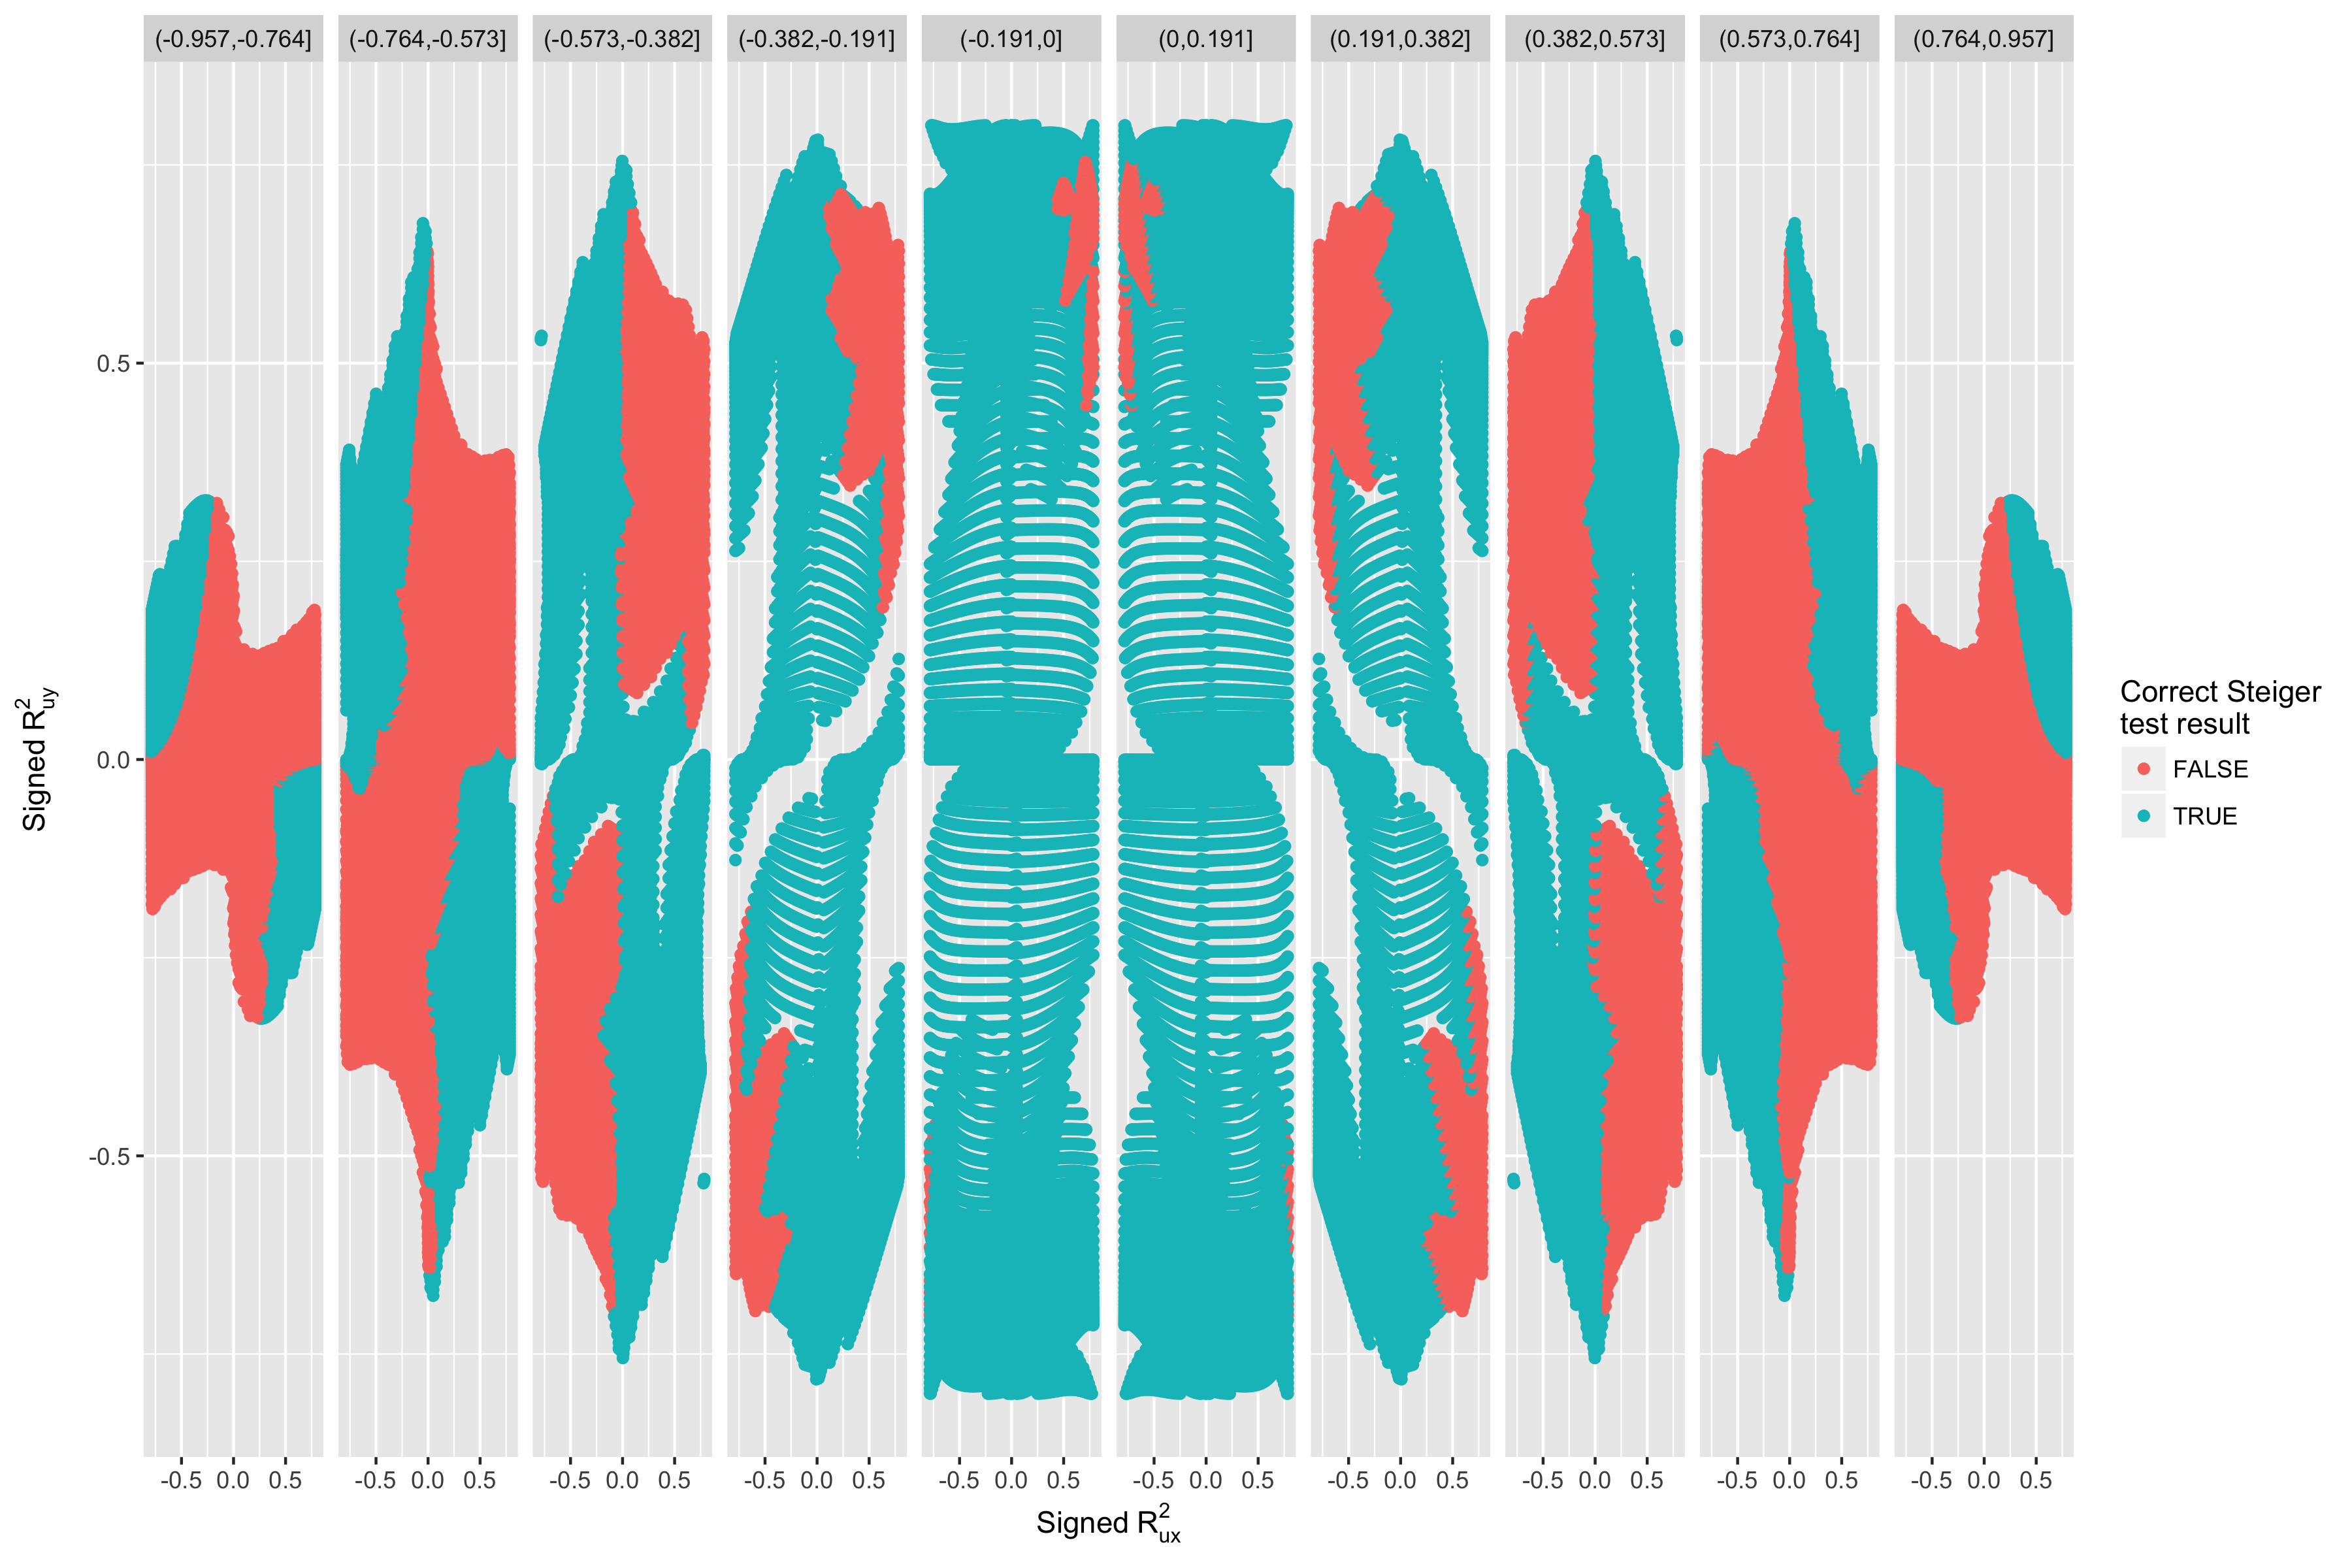
\includegraphics{../images/unmeasured_conf_steiger.png}

Supplementary figure 1: Graph representing the unmeasured confounding
parameters that will lead to the MR Steiger test returning the wrong
causal direction. Columns of boxes represent different signed values of
the observational variance explained between \(x\) and \(y\)
(\(R^2_{xy}\)).


\end{document}
